\documentclass{beamer}
\usepackage[utf8]{inputenc}
\usepackage[T1]{fontenc}
\usepackage[swedish,english]{babel}
\usepackage{color}
\usepackage{xcolor}
\usepackage{amssymb}
\usepackage{amsmath}
\usepackage{ae}
\usepackage{units}
\usepackage{caption}
\usepackage{subcaption}
\usepackage{comment}
\definecolor{olive}{RGB}{0,139,69}
\usetheme{Pittsburgh}
\usecolortheme[RGB={0,139,69}]{structure}
\setbeamertemplate{navigation symbols}{}
\setbeamersize{text margin left=2mm, text margin right=2mm}

%% Skriv \frametitle{foo} för rubrik på en slide
%% \color{olive}{} för text i den gröna färgen
%% Figurer behöver ej vara floats, dvs \begin{figure} ej nödvändigt
%%
%%
%%

\begin{document}

\section{Presentation}

\begin{frame}[label=titleframe]
  \begin{center}

    \textcolor{olive}{{
        \Large Väderparametrars inverkan på \\ energiförluster i en fastighet
      } \\
      - en studie av värmeflöden
    }

    \vskip10pt

    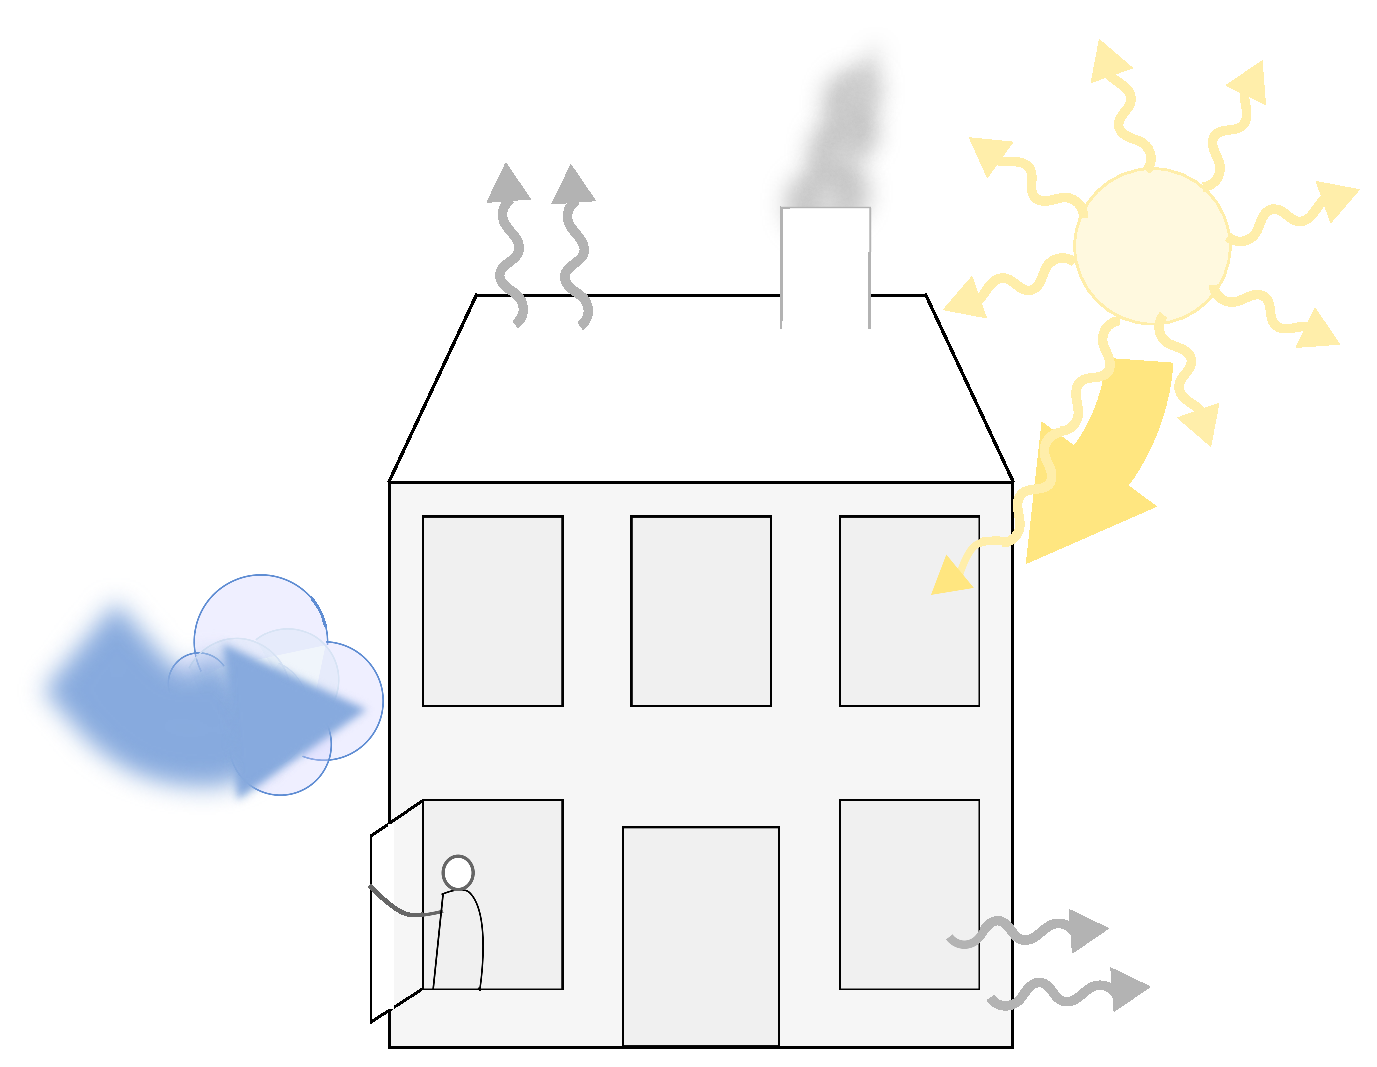
\includegraphics[scale=0.2]{../report/images/hus_framsida.eps}

    \vskip10pt

    Erik Ahlqvist, Ylva Dahl, Mats Lindström, Dan Ståby

    Institutionen för Teknisk Fysik

    29 maj, 2012

  \end{center}
\end{frame}

\subsection{Intro}

\begin{frame}{Presentationsflöde}

\begin{center}
\vskip-10pt
\includegraphics[scale=0.4]{images/upplagg.eps}
\end{center}

\end{frame}


\section{Syfte}
Detta arbete syftar till att undersöka vilka energiförluster en fastighet har och hur dessa påverkas av olika väderrelaterade parametrar, som solinstrålning, utomhustemperatur och vind. Målet är att finna en kvanitativ beskrivning av hur energiflödena in och ut ur fastigheten påverkas av några olika väderparametrar. Primärt kommer vi att undersöka en fastighet på Walleriusgatan i Göteborg, men många av resultaten kommer att kunna appliceras även på andra byggnader.

Beskrivningen av hur vädret påverkar energiflödena skall sedan kunna leda till en modell för hur fastighetens reglerbara energiflöden ska kunna anpassas efter vädret så att en önskad inomhustemperatur bibehålls. I fastigheten som är associerad med projektet finns en väderstation monterad och det är ifrån den väderdata är tänkt att hämtas. Detta ska inte bara ge en trivsammare inomhusmiljö för de boende, utan även en energibesparing för fastigheten. Vi hoppas också kunna ge några byggnadstekniska förslag på åtgärder och kvantifiera hur stora besparingar detta skulle kunna ge – både energimässiga och ekonomiska.

Vi avser att främst bygga vår modell på att luften närmast fastigheten värms upp och bildar ett isolerande lager. Vi kommer också att ta hänsyn till både den fördröjning som sker i fastighetens väggar och den direkta uppvärmning och avkylning som sker med solinstrålning genom fönster respektive ofrivillig ventilation i form av drag.

På sikt hoppas vi att vårt arbete ska leda fram till ett modell som ger ett värde på hur mycket energi som behöver tillföras fastigheten i varje givet ögonblick, beroende på vilka värden väderstationen tidigare har tagit emot. I förlängningen ska detta kunna leda till energibesparande åtgärder för både den här och äldre fastigheter.


\subsection{Byggnadsskal - väggar och tak}

%Definition av h-värde och U-värde

\frame{
       \frametitle{Några definitioner}
        \begin{align*}
        Q &= U\Delta T \\
        Q &= h(T-T_\infty)
        \end{align*}
        \begin{center}
          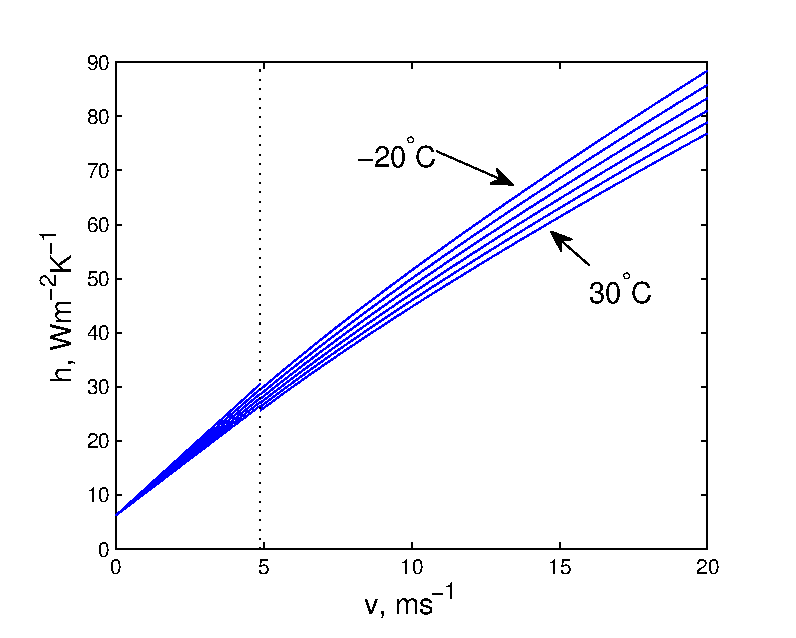
\includegraphics[scale=0.5]{images/hvalues.eps}
        \end{center}
}


%Data för huset

\frame{
       \frametitle{Parametrar för huset}

       \begin{figure}
         \begin{subfigure}[b]{0.48\textwidth}
           \centering
           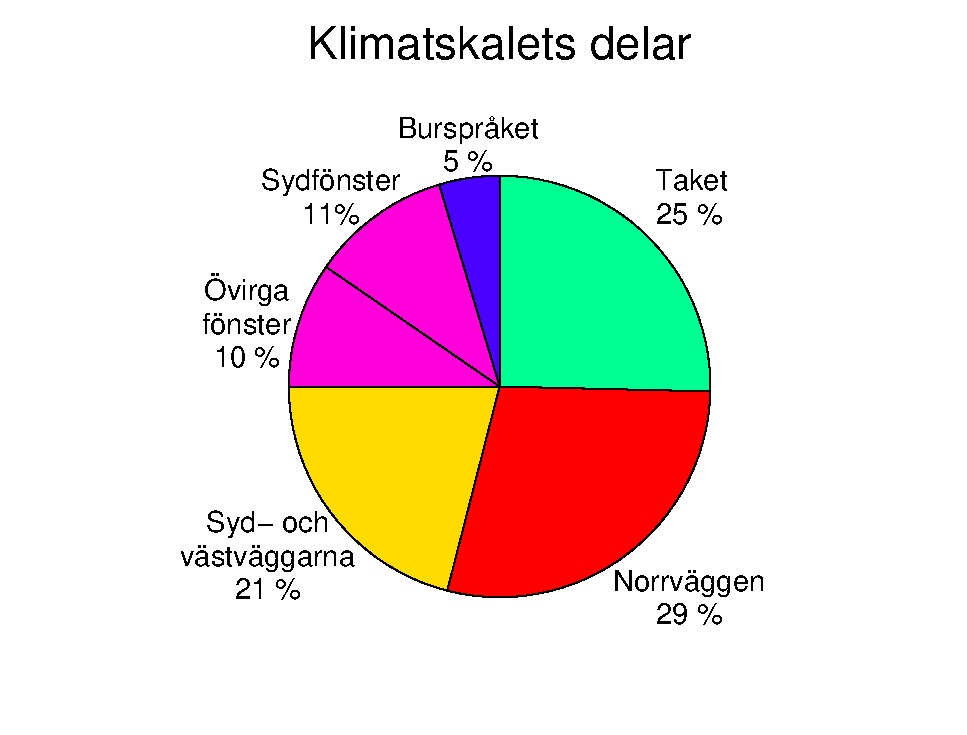
\includegraphics[width=\textwidth]{images/areor_klimatskal.eps}
           \caption*{Total area $\unit[1012]{m^2}$}
         \end{subfigure}
         \begin{subfigure}[b]{0.48\textwidth}
           \centering
           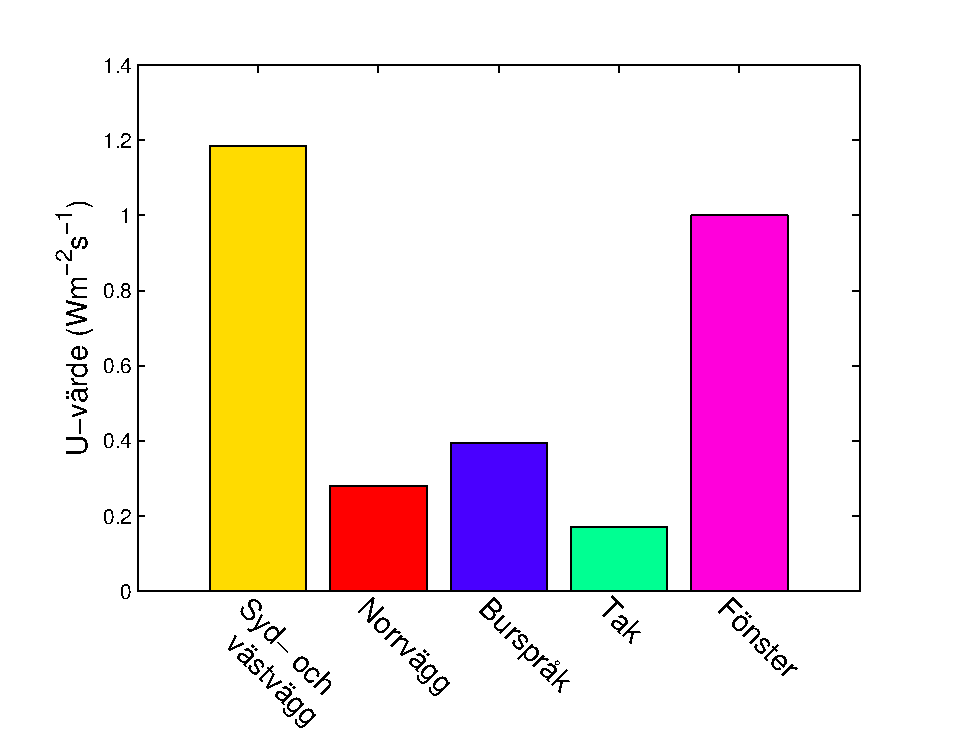
\includegraphics[width=\textwidth]{images/uvalue.eps}
         \end{subfigure}
       \end{figure}
}

\begin{frame}{Problemformulering för väggar och tak}

\begin{align}
k(0)\mathbf{n}\cdot\nabla T(0,t) & = I_{sol}(t) + I_{lv}(T,t) + h(T_\infty-T)
\nonumber \\
T(L,t) & = T_{inne} \nonumber 
\end{align}

\uncover<2>{
\begin{figure}[hbp!]
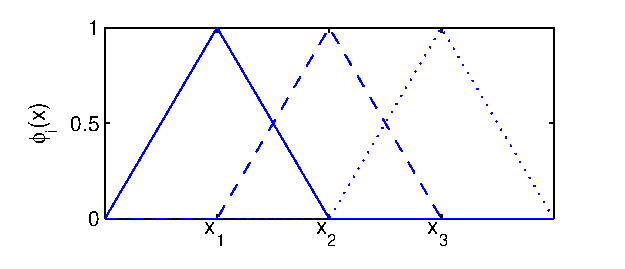
\includegraphics{images/basefun.eps}
\end{figure}
}

\end{frame}

\begin{frame}{Energiflöden, väggar och tak\\En klar decemberdag}
 
\begin{figure}
        \begin{subfigure}[b]{0.48\textwidth}
                \centering
                \includegraphics[width=\textwidth]{images/walls1.eps}
        \end{subfigure}
	\uncover<2>{
        \begin{subfigure}[b]{0.48\textwidth}
                \centering
                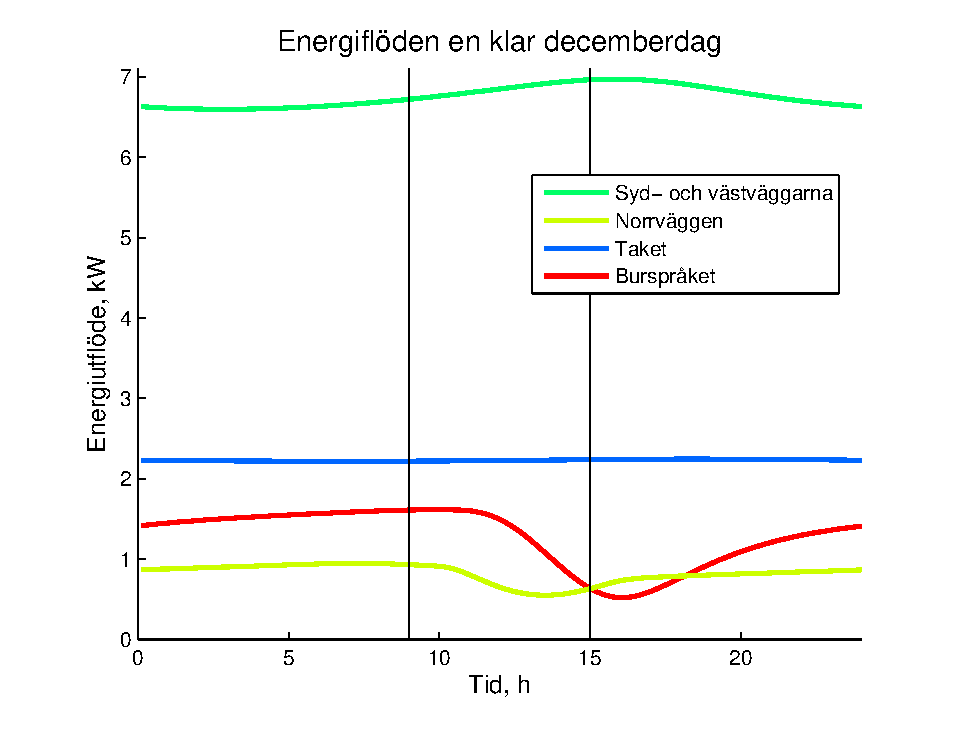
\includegraphics[width=\textwidth]{images/walls2.eps}
        \end{subfigure}
        }
\end{figure}


\end{frame}



\begin{frame}{Infiltrationsförluster}

\begin{figure}[hpbt]
\centering
\includegraphics[width=90mm]{images/pressure3ms.eps}
\caption{\label{fig:windpressure}Vind $\unit[3]{m~s^{-1}}$}
\end{figure}

\end{frame}


\subsection{Grunden}

\begin{frame}{Resultat, grunden\\Hela året}

\begin{figure}[hpbt]
\centering
\includegraphics[height=5cm]{images/foundation.eps}
\caption*{Energiflödet genom grunden}
\end{figure}

\end{frame}

\subsection{Fönster}

\subsubsection{Solens position och intensitet}
\begin{frame}{Solens position}
  \begin{center}
  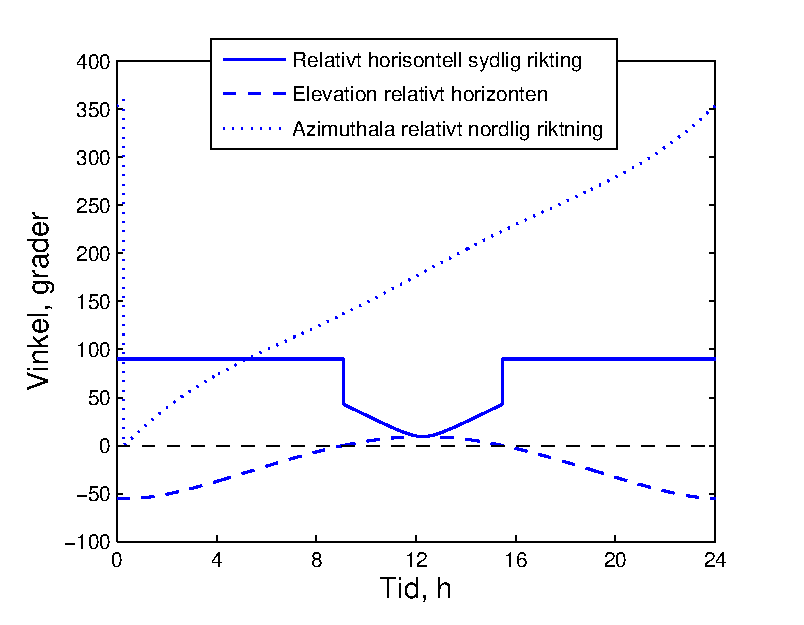
\includegraphics[scale=0.8]{images/sunposition1231.eps}
  \end{center}
\end{frame}

\subsubsection{Direkt strålning, konduktion, konvektion och IR}
\begin{frame}{Flöden genom fönster}
  \begin{columns}
    \begin{column}{.48\textwidth}
      {\small
      \begin{eqnarray*}
        q_{\text{sol}} =  g\left( \theta \right) \cdot I_0 \cos{\left( \theta \right)}\\[10pt]
        g\left( \theta \right) \propto \text{Antal rutor \& beläggningar}\\[10pt]
        \pause q_{\text{kond}} = \frac{1}{\frac{1}{U}+\frac{1}{h}} \left( T_{inne} - T_{ute}\right)\\[10pt]
        \pause q_{\text{långvåg}} = 0,75 \cdot \sigma \left( T_{inne}^4 - T_{ute}^4\right)
      \end{eqnarray*}
      }
    \end{column}
    %\hfill

% Se Karlsson, J. och Roos, A. (2000) för g-värden
% Förklaring av hur vi räknat med S-B:s lag
% Diffus strålning och omedelbar reflektion borträknat

    \begin{column}{.5\textwidth}
      \pause
      \vspace{-30pt}
      \begin{center}
        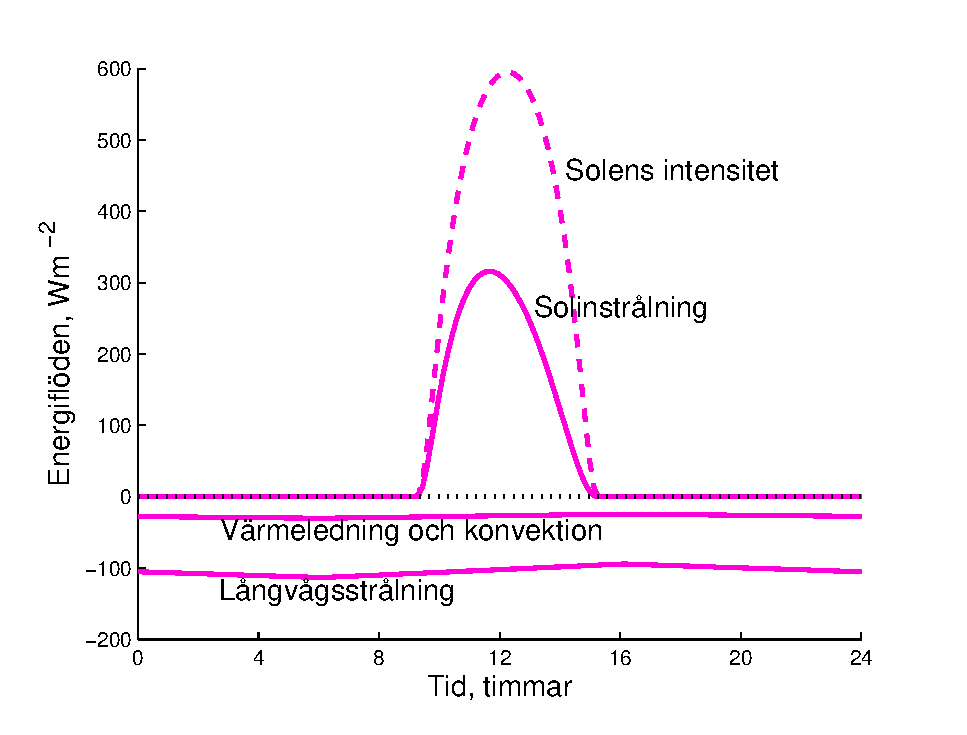
\includegraphics[scale=0.4]{images/windows_flow.eps}
      \end{center}
    \end{column}
  \end{columns}
\end{frame}


\chapter{Slutsats}

%Sammanfattning av resultat

I detta projekt har olika väderparametrars effekt på inomhusklimat och energiåtgång studerats.
Det har framgått att både solinstrålning och infiltrationsförluster på grund av ofrivillig
ventilation kan leda till stora energibidrag. Inom arbetet har även olika förbättringsåtgärder
studerats. Det har visat sig att energibesparingen för att dra nytta av solens värmande effekt kan ge 17~\% lägre energiåtgång över ett soligt dygn, vilket motsvarar 4~\% energibesparing över alla dygn, klara som molnig. Detta kan jämföras med mängden sparad energi för tilläggsisolering för syd- och västväggarna som uppgår till 17~\% av dagens energiåtgång. Det kan också konstateras att de olika väggarna har olika tidskonstanter vilket man måste ta hänsyn till vid regleringen med olika reglersystem för olika delar i byggnaden. Denna effekt kommer dock att minskas något med en tilläggsisolerad av syd- och västväggarna.

Att ta hänsyn till vinden kommer inte nödvändigtvis leda till en lägre energiförbrukning då vinden har en kylande effekt. När det blåser sjunker inomhustemperaturen under önskad temperatur med dagens system om man inte överkompenserar när det inte blåser. Att ta hänsyn till vinden leder dock till en stabilare inomhustemperatur eftersom man eliminerar vindens temperatursänkning.

%Ekonomiska aspekter
Energibesparande åtgärder utöver den direkta styrningen är möjliga att genomföra. För att gå vidare i processen antingen med termostater till alla radiatorer eller tilläggsisolering av ej isolerade fasader behöver föreningen utarbeta en plan för hur de vill att fastigheten ska vara rustad i framtiden. När fasaden behöver renoveras, samt om man får renovera den behöver också besvaras, för att ge tillräcklig information inför en eventuell energibesparande åtgärd. 

Montering av termostater på elementen är billigare än att tilläggsisolera fasaden och enligt beräkningar samt information från leverantörer är det även mer energibesparande. En annan aspekt är att det tillför mervärde för de boende. De boende vill troligtvis kunna reglera temperaturen själva, och vid försäljning av lägenheter bör det kunna ha ökat värdet på desamma.

I samband med en installation av ett reglersystem bör även elektriska termostater installeras, för att minimera tidskonstanterna och för att ge de boende möjligheten att själva bestämma vilken temperatur de vill ha hemma.

%Bevara frågeställningar
Det det har visat sig vara en god idé att ta hänsyn till olika väderparametrar då
detta kan ge en markant besparing under rätt förutsättningar. Självklart är
besparingen olika beroende på fastighetens egenskaper och fastighetens geografiska läge.

%Vad kunde vi inte besvara
Det var svårt att med någon större noggrannhet kvantifiera storleken på de olika energiflödena. Vi
anser dock att våra approximationer ger en god uppfattning om hur stora energiflödena är i förhållande
till varandra. För att få veta exakta värden skulle det vara nödvändigt att implementera de olika
förbättringarna i fastigheten och mäta hur mycket energi som sparats. Alternativt skulle
bättre modeller kunna ge en exaktare bild. Problemet med det är att mer komplexa modeller tenderar att
bli mer beräkningsintensiva.



\subsection{Avslutande sammanfattning}

\frame{
\begin{center}
  \Huge{Väderstation?}
\end{center}
        \vskip1.3cm
\uncover<2>{
\begin{center}
  \color{magenta}{\Huge{Det finns bättre alternativ!}}
\end{center}

}
}

\againframe{titleframe}

\end{document}
